%review=doublespace preprint=single 5p=2 column
\documentclass[12pt,3p,authoryear]{elsarticle}

%% add packages %%
%% ------------ %%
\usepackage[hyphens]{url}
\usepackage{graphicx}
\usepackage{booktabs}
\usepackage[T1]{fontenc}
\usepackage{lmodern}
\usepackage{caption}
\usepackage{subfig}
\usepackage{amssymb, amsmath}
\usepackage[inline]{enumitem}
\usepackage{float}
\usepackage{tabularx}
\usepackage[dvipsnames, table]{xcolor}
\usepackage{ifxetex, ifluatex}
\usepackage{fixltx2e}
\usepackage[unicode=true, colorlinks]{hyperref}
\usepackage{cleveref}
\usepackage{tabu}
\usepackage{mathpazo}
%% ------------ %%

%% Conditional Packages %%
%% -------------------- %%

\usepackage{easyReview}



% use upquote if available, for straight quotes in verbatim environments
\IfFileExists{upquote.sty}{\usepackage{upquote}}{}

\ifnum 0\ifxetex 1\fi\ifluatex 1\fi=0 % if pdftex
  \usepackage[utf8]{inputenc}


\else % if luatex or xelatex
  \usepackage{fontspec}
  \ifxetex
    \usepackage{xltxtra,xunicode}
  \fi
  \defaultfontfeatures{Mapping=tex-text,Scale=MatchLowercase}
  \newcommand{\euro}{€}



    \setmonofont{sourcecodepro}


\fi

% use microtype if available
\IfFileExists{microtype.sty}{\usepackage{microtype}}{}




\usepackage{color}
\usepackage{fancyvrb}
\newcommand{\VerbBar}{|}
\newcommand{\VERB}{\Verb[commandchars=\\\{\}]}
\DefineVerbatimEnvironment{Highlighting}{Verbatim}{commandchars=\\\{\}}
% Add ',fontsize=\small' for more characters per line
\usepackage{framed}
\definecolor{shadecolor}{RGB}{248,248,248}
\newenvironment{Shaded}{\begin{snugshade}}{\end{snugshade}}
\newcommand{\AlertTok}[1]{\textcolor[rgb]{0.94,0.16,0.16}{#1}}
\newcommand{\AnnotationTok}[1]{\textcolor[rgb]{0.56,0.35,0.01}{\textbf{\textit{#1}}}}
\newcommand{\AttributeTok}[1]{\textcolor[rgb]{0.77,0.63,0.00}{#1}}
\newcommand{\BaseNTok}[1]{\textcolor[rgb]{0.00,0.00,0.81}{#1}}
\newcommand{\BuiltInTok}[1]{#1}
\newcommand{\CharTok}[1]{\textcolor[rgb]{0.31,0.60,0.02}{#1}}
\newcommand{\CommentTok}[1]{\textcolor[rgb]{0.56,0.35,0.01}{\textit{#1}}}
\newcommand{\CommentVarTok}[1]{\textcolor[rgb]{0.56,0.35,0.01}{\textbf{\textit{#1}}}}
\newcommand{\ConstantTok}[1]{\textcolor[rgb]{0.00,0.00,0.00}{#1}}
\newcommand{\ControlFlowTok}[1]{\textcolor[rgb]{0.13,0.29,0.53}{\textbf{#1}}}
\newcommand{\DataTypeTok}[1]{\textcolor[rgb]{0.13,0.29,0.53}{#1}}
\newcommand{\DecValTok}[1]{\textcolor[rgb]{0.00,0.00,0.81}{#1}}
\newcommand{\DocumentationTok}[1]{\textcolor[rgb]{0.56,0.35,0.01}{\textbf{\textit{#1}}}}
\newcommand{\ErrorTok}[1]{\textcolor[rgb]{0.64,0.00,0.00}{\textbf{#1}}}
\newcommand{\ExtensionTok}[1]{#1}
\newcommand{\FloatTok}[1]{\textcolor[rgb]{0.00,0.00,0.81}{#1}}
\newcommand{\FunctionTok}[1]{\textcolor[rgb]{0.00,0.00,0.00}{#1}}
\newcommand{\ImportTok}[1]{#1}
\newcommand{\InformationTok}[1]{\textcolor[rgb]{0.56,0.35,0.01}{\textbf{\textit{#1}}}}
\newcommand{\KeywordTok}[1]{\textcolor[rgb]{0.13,0.29,0.53}{\textbf{#1}}}
\newcommand{\NormalTok}[1]{#1}
\newcommand{\OperatorTok}[1]{\textcolor[rgb]{0.81,0.36,0.00}{\textbf{#1}}}
\newcommand{\OtherTok}[1]{\textcolor[rgb]{0.56,0.35,0.01}{#1}}
\newcommand{\PreprocessorTok}[1]{\textcolor[rgb]{0.56,0.35,0.01}{\textit{#1}}}
\newcommand{\RegionMarkerTok}[1]{#1}
\newcommand{\SpecialCharTok}[1]{\textcolor[rgb]{0.00,0.00,0.00}{#1}}
\newcommand{\SpecialStringTok}[1]{\textcolor[rgb]{0.31,0.60,0.02}{#1}}
\newcommand{\StringTok}[1]{\textcolor[rgb]{0.31,0.60,0.02}{#1}}
\newcommand{\VariableTok}[1]{\textcolor[rgb]{0.00,0.00,0.00}{#1}}
\newcommand{\VerbatimStringTok}[1]{\textcolor[rgb]{0.31,0.60,0.02}{#1}}
\newcommand{\WarningTok}[1]{\textcolor[rgb]{0.56,0.35,0.01}{\textbf{\textit{#1}}}}


\usepackage{longtable}




% Pandoc toggle for numbering sections (defaults to be off)
\setcounter{secnumdepth}{5}

%% Use Landscape Pages
\usepackage{lscape}

\usepackage{setspace}
\setstretch{1.5}

\usepackage{lmodern}

%% -------------------- %%

%% Create and Provide some customizations %%
%% -------------------------------------- %%
\providecommand{\tightlist}{%
  \setlength{\itemsep}{0pt}\setlength{\parskip}{0pt}}
  
%% Custom macros
\newtheorem{mydef}{Definition}
\newcommand{\bs}[1]{\ensuremath{\boldsymbol{#1}}}
\newcommand{\diag}[1]{\mathrm{diag}\left(#1\right)}
\newcommand{\seq}[3][1]{\ensuremath{#2_{#1},\ldots,\,#2_{#3}}}
\newcommand{\note}[1]{\marginpar{\scriptsize\tt{\color{RoyalBlue}#1}}}
\newcommand{\edit}[1]{{\color{OrangeRed} #1}}

% set some lengths
\setlength{\parindent}{0pt}
% \setlength{\parskip}{6pt plus 2pt minus 1pt}
\setlength{\emergencystretch}{3em}  % prevent overfull lines

%% Hyperref color setup
\AtBeginDocument{%
  %% Define Colors
  \newcommand\myshade{80}
  \colorlet{mylinkcolor}{violet!\myshade!black}
  \colorlet{mycitecolor}{YellowOrange!\myshade!black}
  \colorlet{myurlcolor}{Aquamarine!\myshade!black}

  \hypersetup{
    breaklinks = true,
    bookmarks  = true,
    pdfauthor  = {},
    pdftitle   = {Comparison of Multivariate Prediction Methods},
    linkcolor  = mylinkcolor,
    citecolor  = mycitecolor,
    urlcolor   = myurlcolor,
    colorlinks = true,
  }
}
\urlstyle{same}  % don't use monospace font for urls
%% -------------------------------------- %%

%% Customizations %%
%% -------------- %%
 % turn line numbering on

%% -------------- %%

%% Configure Bibliography %%
%% ---------------------- %%
\bibliographystyle{elsarticle-harv}
\biboptions{numbers,sort&compress}

\makeatletter
\providecommand{\doi}[1]{%
  \begingroup
    \let\bibinfo\@secondoftwo
    \urlstyle{rm}%
    \href{http://dx.doi.org/#1}{%
      doi:\discretionary{}{}{}%
      \nolinkurl{#1}%
    }%
  \endgroup
}
\makeatother

% 

%% Header Includes %%
%% --------------- %%
%% --------------- %%



\begin{document}
%% --- Front Matter Start --- %%
\begin{frontmatter}

  \title{Comparison of Multivariate Prediction Methods}
  
    \author[KBM]{Raju Rimal\corref{c1}}
   \ead{raju.rimal@nmbu.no} 
   \cortext[c1]{Corresponding Author}
    \author[KBM]{Trygve Almøy}
   \ead{trygve.almoy@nmbu.no} 
  
    \author[NMBU]{Solve Sæbø}
   \ead{solve.sabo@nmbu.no} 
  
      \address[KBM]{Faculty of Chemistry and Bioinformatics, Norwegian University of Life
Sciences, Ås, Norway}
    \address[NMBU]{Prorector, Norwegian University of Life Sciences, Ås, Norway}
  
  \begin{abstract}
  While Data science is battling to extract information from the enormous
  explosion of data, many estimators and algorithms are being developed
  for better prediction. Researchers and data scientists often introduce
  new methods and evaluate them based on various aspects of data. However,
  studies on the impact of/on model with multiple response model is
  limited. This study compares some newly-developed (envelope) and
  well-established (PLS, PCR) prediction methods based on simulated data
  specifically designed by varying properties such as multicollinearity,
  correlation between multiple responses and amount of information content
  in predictor variables. This study aims to give some insight on these
  methods and help researcher to understand and use them for further
  study.
  \end{abstract}
   \begin{keyword} model-comparison,multi-response,simrel\end{keyword}

\end{frontmatter}

\hypertarget{introduction}{%
\section{Introduction}\label{introduction}}

Prediction has been an essential components of modern data science,
weather it is statistical analysis or machine learning. Modern
technology has facilitated a massive explosion of data, however, such
data often contain irrelevant information consequently making prediction
difficult. Researchers are devising new methods and algorithms in order
to extract information to create robust predictive models. Mostly such
models contain predictor variables that are directly or indirectly
correlated with other predictor variables. In addition studies often
constitute of many response variables correlated with each other. These
interlinked relationships influence any study, whether it is predictive
modeling or inference.

Modern inter-disciplinary research fields such as chemometrics,
econometrics and bioinformatics are handling multi-response models
extensively. This paper attempts to compare some multivariate prediction
methods based on their prediction performance on linear model data with
specific properties. The properties includes correlation between
response variables, correlation between predictor variables, number of
predictor variables and the position of relevant predictor components.
These properties are discussed more in the
\protect\hyperlink{experimental-design}{Experimental Design} section.
\citet{saebo2015simrel} and \citet{Alm_y_1996} have made a similar
comparison in the single response setting. In addition,
\citet{Rimal2018} has also made a basic comparison on some prediction
methods and their interaction with the data properties of a
multi-response model. The main aim of this paper is to present a
comprehensive comparison of contemporary prediction methods such as
simultaneous envelope estimation (Senv) \citep{cook2015simultaneous} and
envelope estimation in predictor space (Xenv) \citep{cook2010envelope}
with customary prediction methods such as Principal Component Regression
(PCR), Partial Least Squares Regression (PLS) using simulated dataset
with controlled properties. An experimental design and the methods under
comparison are discussed further, followed by a brief discussion of the
strategy behind the data simulation.

\hypertarget{simulation-model}{%
\section{Simulation Model}\label{simulation-model}}

Consider a model where the response vector \((\mathbf{y})\) with \(m\)
elements and predictor vector \((\mathbf{x})\) with \(p\) elements
follow a multivariate normal distribution as follows,

\begin{equation}
  \begin{bmatrix}
    \mathbf{y} \\ \mathbf{x}
  \end{bmatrix} \sim \mathcal{N}
  \left(
    \begin{bmatrix}
      \boldsymbol{\mu}_y \\
      \boldsymbol{\mu}_x
    \end{bmatrix},
    \begin{bmatrix}
    \boldsymbol{\Sigma}_{yy} & \boldsymbol{\Sigma}_{yx} \\
    \boldsymbol{\Sigma}_{xy} & \boldsymbol{\Sigma}_{xx}
    \end{bmatrix}
  \right)
  \label{eq:model-1}
\end{equation}

where, \(\boldsymbol{\Sigma}_{yy}\) and \(\boldsymbol{\Sigma}_{xx}\) are
the variance-covariance matrices of \(\mathbf{y}\) and \(\mathbf{x}\),
respectively, \(\boldsymbol{\Sigma}_{xy}\) is the covariance between
\(\mathbf{x}\) and \(\mathbf{y}\) and \(\boldsymbol{\mu}_y\) and
\(\boldsymbol{\mu}_x\) are mean vectors of \(\mathbf{x}\) and
\(\mathbf{y}\), respectively. A linear model based on \eqref{eq:model-1}
is,

\begin{equation}
\mathbf{y} = \boldsymbol{\mu}_y + 
  \boldsymbol{\beta}^t(\mathbf{x} - \boldsymbol{\mu_x}) + 
  \boldsymbol{\epsilon}
\label{eq:reg-model-1}
\end{equation} where, \(\underset{m\times p}{\boldsymbol{\beta}^t}\) is
a matrix of regression coefficients and \(\boldsymbol{\epsilon}\) is an
error term such that
\(\boldsymbol{\epsilon} \sim \mathcal{N}(0, \boldsymbol{\Sigma}_{y|x})\)

In a model like \eqref{eq:reg-model-1}, we assume that the variation in
response \(\mathbf{y}\) is partly explained by the predictor
\(\mathbf{x}\). However, in many situations, only a subspace of the
predictor space is relevant for the variation in the response
\(\mathbf{y}\). This space can be referred to as the relevant space of
\(\mathbf{x}\) and the rest as irrelevant space. In the similar manner,
we can assume that a subset of the response space contains the
information that the predictors can explain for a given model
(Figure-\ref{fig:relevant-space}). \citet{cook2010envelope} and
\citet{cook2015simultaneous} have referred to the relevant space as
material space, and the irrelevant space as immaterial space.

\begin{figure}

{\centering 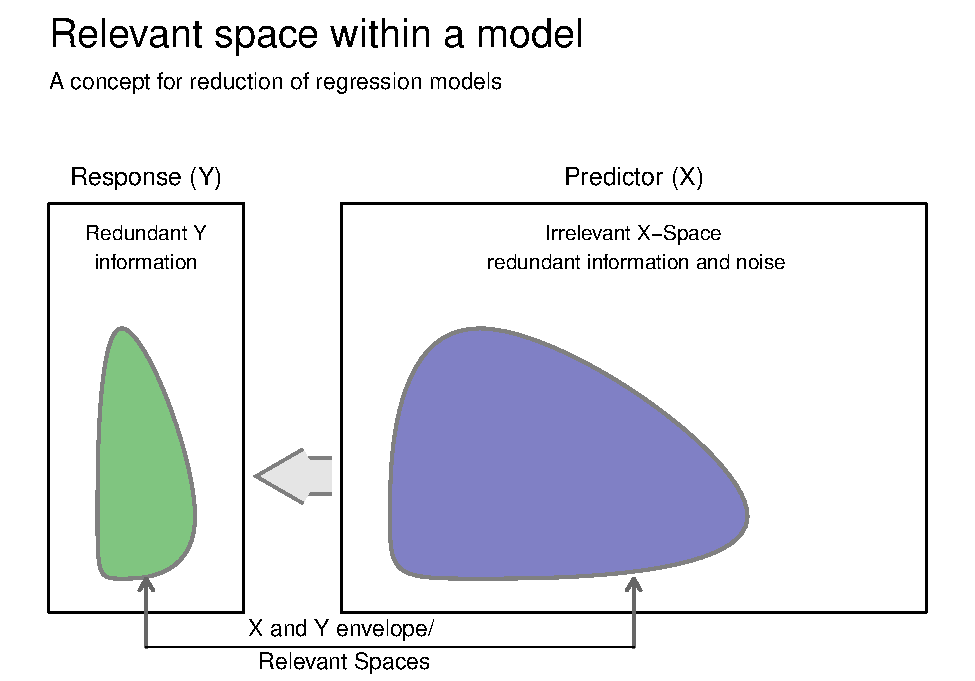
\includegraphics[width=0.8\linewidth]{main_files/figure-latex/relevant-space-1} 

}

\caption{Relevant space in a regression model}\label{fig:relevant-space}
\end{figure}

With an orthogonal transformation of \(\mathbf{y}\) and \(\mathbf{x}\)
to latent variables \(\mathbf{w}\) and \(\mathbf{z}\), respectively, by
\(\mathbf{w=Qy}\) and \(\mathbf{z = Rx}\), where \(\mathbf{Q}\) and
\(\mathbf{R}\) are orthogonal rotation matrices, an equivalent model to
\eqref{eq:reg-model-1} in terms of the latent variables can be written as,

\begin{equation}
\mathbf{w} = \boldsymbol{\mu}_w + \boldsymbol{\alpha}^t(\mathbf{z} - \boldsymbol{\mu_z}) + \boldsymbol{\tau}
\label{eq:reg-model-2}
\end{equation} where, \(\underset{m\times p}{\boldsymbol{\alpha}^t}\) is
a matrix of regression coefficients and \(\boldsymbol{\tau}\) is an
error term such that
\(\boldsymbol{\tau} \sim \mathcal{N}(0, \boldsymbol{\Sigma}_{w|z})\).
Model \eqref{eq:reg-model-2} follows the distribution,

\begin{equation}
  \begin{bmatrix}
    \mathbf{w} \\ \mathbf{z}
  \end{bmatrix} \sim \mathcal{N}
  \left(
    \begin{bmatrix}
      \boldsymbol{\mu}_w \\
      \boldsymbol{\mu}_z
    \end{bmatrix},
    \begin{bmatrix}
    \boldsymbol{\Sigma}_{ww} & \boldsymbol{\Sigma}_{wz} \\
    \boldsymbol{\Sigma}_{zw} & \boldsymbol{\Sigma}_{zz}
    \end{bmatrix}
  \right)
  \label{eq:model-2}
\end{equation}

where, \(\boldsymbol{\Sigma}_{ww}\) and \(\boldsymbol{\Sigma}_{zz}\) are
the variance-covariance matrices of \(\mathbf{w}\) and \(\mathbf{z}\),
respectively. \(\boldsymbol{\Sigma}_{zw}\) is the covariance between
\(\mathbf{z}\) and \(\mathbf{w}\). \(\boldsymbol{\mu}_w\) and
\(\boldsymbol{\mu}_z\) are mean vector of \(\mathbf{z}\) and
\(\mathbf{w}\) respectively.

Here, the elements of \(\mathbf{w}\) and \(\mathbf{z}\) are the
principal components of responses and predictors, which will
respectively be referred as ``response components'' and ``predictor
components''. The column vectors of respective rotation matrices
\(\mathbf{Q}\) and \(\mathbf{R}\) are the eigenvectors corresponding to
these principal components.

Following the concept of relevant space, a subset of predictor
components can be imagined to span the predictor space. These components
can be regarded as relevant predictor components. \citet{Naes1985}
introduced the concept of relevant components which was explored further
by \citet{helland1990partial}, \citet{naes1993relevant},
\citet{Helland1994b} and \citet{Helland2000}. The corresponding
eigenvectors were referred to as relevant eigenvectors. A similar logic
is introduced by \citet{cook2010envelope} and later by
\citet{cook2013envelopes} as an envelope which is the space spanned by
the relevant eigenvectors \citep[pp.~101]{cook2018envelope}.

In addition, various simulation studies have been performed with the
model based on the concept of relevant subspace. A simulation study by
\citet{Alm_y_1996} has used a single response simulation model based on
reduced regression and has compared some contemporary multivariate
estimators. In the recent years \citet{helland2012near},
\citet{saebo2015simrel}, \citet{helland2016algorithms} and
\citet{Rimal2018} implemented similar simulation examples as we are
discussing in this study. This paper, however, presents an extensive
simulation study based on multi-response data simulated with
experimental design and compares relatively new methods such as
simultaneous envelopes with well established methods such as partial
least squares and principal components regression. \citet{Rimal2018} has
a detail discussion about the simulation model that we have opted here.
The following section presents the estimators under comparison in more
detail.

\hypertarget{prediction-methods}{%
\section{Prediction Methods}\label{prediction-methods}}

Partial least squares regression (PLS) and Principal component
regression (PCR) has been used in many disciplines such as chemometrics,
econometrics, bioinformatics and machine learning, where wide predictor
matrices, i.e. \(p\) (number or predictors) \textgreater{} \(n\) (number
of observation) is common. These methods are popular in multivariate
analysis, especially for exploratory studies and prediction.

In recent years, a concept of envelope introduced by \citet{Cook2007a}
based on reduction in regression model has been implemented for the
development of envelope estimation in the subsequent papers.

In this study, we will follow estimation methods based on their
prediction performance on data simulated with different controlled
properties.

\begin{description}
\tightlist
\item[\emph{Principal Components Regression (PCR):}]
Principal components are the linear combinations of predictor variables
such that the transformation makes the new variables uncorrelated and
the variation of the original dataset captured by them are ordered. In
other words, each successive components captures maximum variation left
by the preceding components in predictor variables \citep{Jolliffe2002}.
Principal components regression uses these principal components to
explain the variation in the response.
\item[\emph{Partial Least Squares (PLS):}]
Two variants of PLS: PLS1 and PLS2 will be used for comparison. The
first one considers individual response variables separately, i.e.~each
response is predicted with a single response model, while the latter
considers all response variables together. In PLS regression the
components are determined such as to maximize a covariance between
response and predictors \citep{DeJong1993}.
\item[\emph{Envelopes:}]
The envelope, introduced by \citet{Cook2007a}, was first used as a
response envelope \citep{cook2010envelope} as a smallest subspace
\(\mathcal{E}\) in the response space such that the span of regression
coefficients lies in that space. Since a multivariate linear regression
model contains relevant (material) and irrelevant (immaterial) variation
in both response and predictor, the relevant part provides information,
while irrelevant part increases the estimative variation. The concept of
envelope uses the relevant part for estimation while excluding the
irrelevant part consequently increasing the efficiency of the model
\citep{cook2016algorithms}.

The concept was later extended to the predictor space, where the
predictor envelope was defined \citep{cook2013envelopes}. Further
\citet{cook2015simultaneous} uses envelopes for joint reduction of the
responses and predictors and argued to produce efficiency gains greater
than using individual envelops either of the response and predictors.
All the variants of envelope estimations are based on maximum likelihood
estimation. Here in this study we will also use predictor envelope
(Xenv) and simultaneous envelope (Senv) for the comparison.
\end{description}

\hypertarget{modification-in-envelope-estimation}{%
\subsection{Modification in envelope
estimation}\label{modification-in-envelope-estimation}}

Since envelope estimators (Xenv and Senv) are based on maximum
likelihood estimation (MLE), it fails to estimate in case of wide
matrices, i.e. \(p > n\). In order to incorporate these methods in our
comparison, we have used the principal components \((\mathbf{z})\) of
the predictor variables \((\mathbf{x})\) as predictors, using the
required number of components for capturing 97.5\% of the variation in
\(\mathbf{x}\). The new set of variables, \(\mathbf{z}\), were used for
envelope estimation. The regression coefficients
\((\hat{\boldsymbol{\alpha}})\) corresponding to these new variables
\(\mathbf{z}\) were transformed back to obtain coefficients for each
predictor variable as,

\[\hat{\boldsymbol{\beta}} = \mathbf{e}_k\hat{\boldsymbol{\alpha}_k}\]
where, \(\mathbf{e}_k\) is the eigenvectors with \(k\) number of
components.

\hypertarget{experimental-design}{%
\section{Experimental Design}\label{experimental-design}}

This study compares prediction methods based on their prediction
ability. Data with specific properties are simulated, some of which are
easier to predict than others. These data are simulated using the
R-package \texttt{simrel}, which is discussed in \citet{saebo2015simrel}
and \citet{Rimal2018}. Here we will use four different factors to vary
the property of the data: a) Number of predictors (\texttt{p}), b)
Multicollinearity in predictor variables (\texttt{gamma}), c)
Correlation in response variables (\texttt{eta}) and d) position of
predictor components relevant for the response (\texttt{relpos}). Using
two levels of \texttt{p}, \texttt{gamma} and \texttt{relpos} and four
levels of \texttt{eta}, 32 set of distinct properties are designed for
the simulation.

\begin{description}
\item[\textbf{Number of predictors:}]
In order to observe the performance of the methods on tall and wide
predictor matrices, 20 and 250 predictor variables are simulated.
Parameter \texttt{p} controls this properties in the \texttt{simrel}
function.
\item[\textbf{Multicollinearity in predictor variables:}]
Highly collinear predictors can be explained completely by few
components. The parameter \texttt{gamma} (\(\gamma\)) in \texttt{simrel}
controls decline in the eigenvalues of the predictor variables as
\eqref{eq:gamma}.

\begin{equation}
  \lambda_i = e^{-\gamma(i - 1)}, \gamma > 0 \text{ and } i = 1, 2, \ldots, p
  \label{eq:gamma}
  \end{equation}
\end{description}

Here, \(\lambda_i, i = 1, 2, \ldots p\) are eigenvalues of the predictor
variables. Here we have used 0.2 and 0.9 as different levels of
\texttt{gamma}. The higher the value of gamma, the higher will be the
correlation between predictors and vice versa.

\begin{description}
\item[\textbf{Correlation in response variables:}]
Correlation among response variables is a less explored area. Here we
have tried to explore that part with 4 levels of correlation in the
response variables. We have used the \texttt{eta} (\(\eta\)) parameter
of \texttt{simrel} for controlling the decline in eigenvalues
corresponding to the response variables as \eqref{eq:eta}.

\begin{equation}
  \kappa_i = e^{-\eta(i - 1)}, \eta > 0 \text{ and } j = 1, 2, \ldots, m
  \label{eq:eta}
\end{equation}
\end{description}

Here, \(\kappa_i, i = 1, 2, \ldots m\) are the eigenvalues of the
response variables and \texttt{m} is the number of response variables.
Here we have used 0, 0.4, 0.8 and 1.2 as different levels of
\texttt{eta}. The larger the value of eta, the larger will be the
correlation between response variables and vice versa.

\begin{description}
\tightlist
\item[\textbf{Position of predictor components relevant to the
response:}]
The principal components of the predictors are ordered. The first
principal component captures most of the variation in the predictors.
The second captures the most in the rest that is left by the first
principal components and so on. In highly collinear predictors, the
variation captured by the first few components is relatively high.
However, if those components are not relevant for the response,
prediction becomes difficult \citep{Helland1994b}. Here, two levels of
the positions of these relevant components are used: 1, 2, 3, 4 and 5,
6, 7, 8.
\end{description}

Further, a complete factorial design from the levels of the above given
parameters gave us 32 designs. Each design is associated with a dataset
having unique properties. Figure\textasciitilde{}\ref{fig:design-plot},
shows all the designs. For each design and prediction method, 50
datasets were simulated for replication. In total, there were
\(5 \times 32 \times 50\), i.e.~8000 dataset simulated.

\begin{figure}
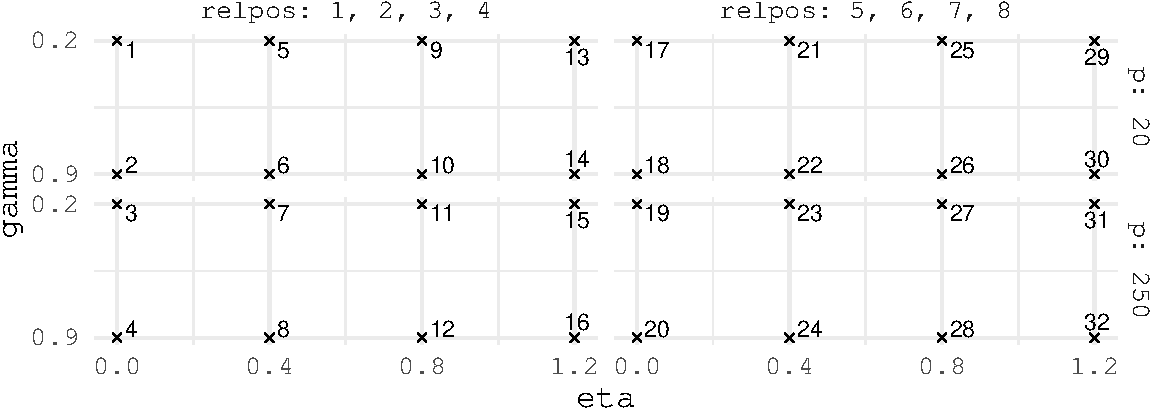
\includegraphics[width=1\linewidth]{main_files/figure-latex/design-plot-1} \caption{Experimental Design of simulation parameters. Each point represents an unique data property.}\label{fig:design-plot}
\end{figure}

\begin{description}
\tightlist
\item[\textbf{Common parameters:}]
Each dataset was simulated with \(n = 100\) number of observation and
\(m = 4\) response variables. Further, the coefficient of determination
corresponding to each response components in all the designs is set to
and 0.8. In addition, we have assumed that there is only one informative
response component. Hence, the informative response component is rotated
orthogonally together with three uninformative response components to
generate four response variables. This spread out the information in all
simulated response variables. For further details on the simulation tool
see \citep{Rimal2018}.
\end{description}

An example of simulation parameters for the first design is as follows:

\begin{Shaded}
\begin{Highlighting}[]
\KeywordTok{simrel}\NormalTok{(}
    \DataTypeTok{n       =} \DecValTok{100}\NormalTok{,                 }\CommentTok{## Training samples}
    \DataTypeTok{p       =} \DecValTok{20}\NormalTok{,                  }\CommentTok{## Predictors}
    \DataTypeTok{m       =} \DecValTok{4}\NormalTok{,                   }\CommentTok{## Responses}
    \DataTypeTok{q       =} \DecValTok{20}\NormalTok{,                  }\CommentTok{## Relevant predictors}
    \DataTypeTok{relpos  =} \KeywordTok{list}\NormalTok{(}\KeywordTok{c}\NormalTok{(}\DecValTok{1}\NormalTok{, }\DecValTok{2}\NormalTok{, }\DecValTok{3}\NormalTok{, }\DecValTok{4}\NormalTok{)), }\CommentTok{## Relevant predictor components index}
    \DataTypeTok{eta     =} \DecValTok{0}\NormalTok{,                   }\CommentTok{## Decay factor of response eigenvalues}
    \DataTypeTok{gamma   =} \FloatTok{0.2}\NormalTok{,                 }\CommentTok{## Decay factor of predictor eigenvalues}
    \DataTypeTok{R2      =} \FloatTok{0.8}\NormalTok{,                 }\CommentTok{## Coefficient of determination}
    \DataTypeTok{ypos    =} \KeywordTok{list}\NormalTok{(}\KeywordTok{c}\NormalTok{(}\DecValTok{1}\NormalTok{, }\DecValTok{2}\NormalTok{, }\DecValTok{3}\NormalTok{, }\DecValTok{4}\NormalTok{)),}
    \DataTypeTok{type    =} \StringTok{"multivariate"}
\NormalTok{)}
\end{Highlighting}
\end{Shaded}

\begin{figure}
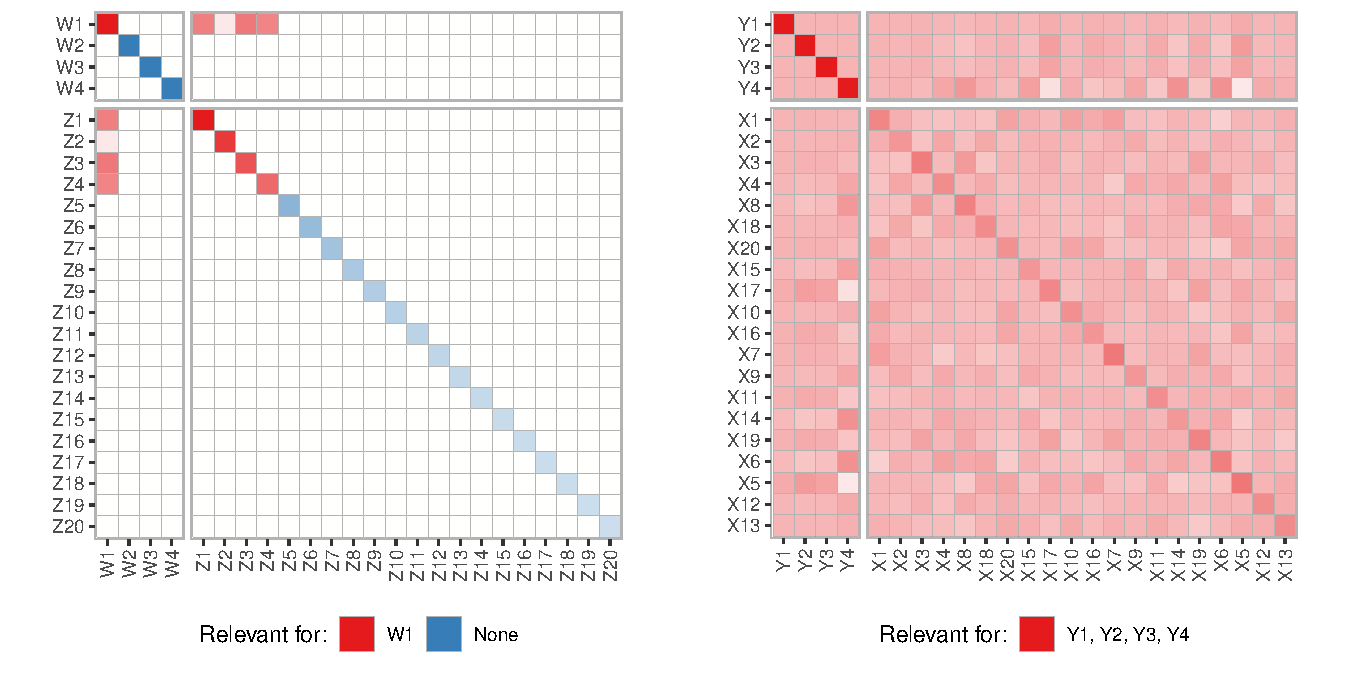
\includegraphics[width=1\linewidth]{main_files/figure-latex/cov-plot-1-1} \caption{(left) Covariance structure of latent components. (right) Covariance structure of predictor and response}\label{fig:cov-plot-1}
\end{figure}

Figure \ref{fig:cov-plot-1} shows the covariance structure of the data
simulated with this design. The figure shows that the predictor
components at position 1, 2, 3 and 4 are relevant for the first response
component. After the rotation with orthogonal rotation matrix, all
predictors are somewhat relevant for all response variables, fulfilling
other desired properties like multicollinearity and coefficient of
determination. For this same design, Figure \ref{fig:est-cov-plot}(top
left) shows that the predictor components 1, 2, 3 and 4 are relevant for
the first response component. All other predictor components are
irrelevant and all other response components are uninformative. However,
due to orthogonal rotation of the informative response component
together with uninformative response components, all response variables
in the population have similar covariance with the relevant predictor
components (Figure \ref{fig:est-cov-plot}(top right)). The sample
covariances between the predictors components and predictor variables
with response variables are in Figure \ref{fig:est-cov-plot} (bottom
left) and (bottom right) respectively.










\begin{figure}
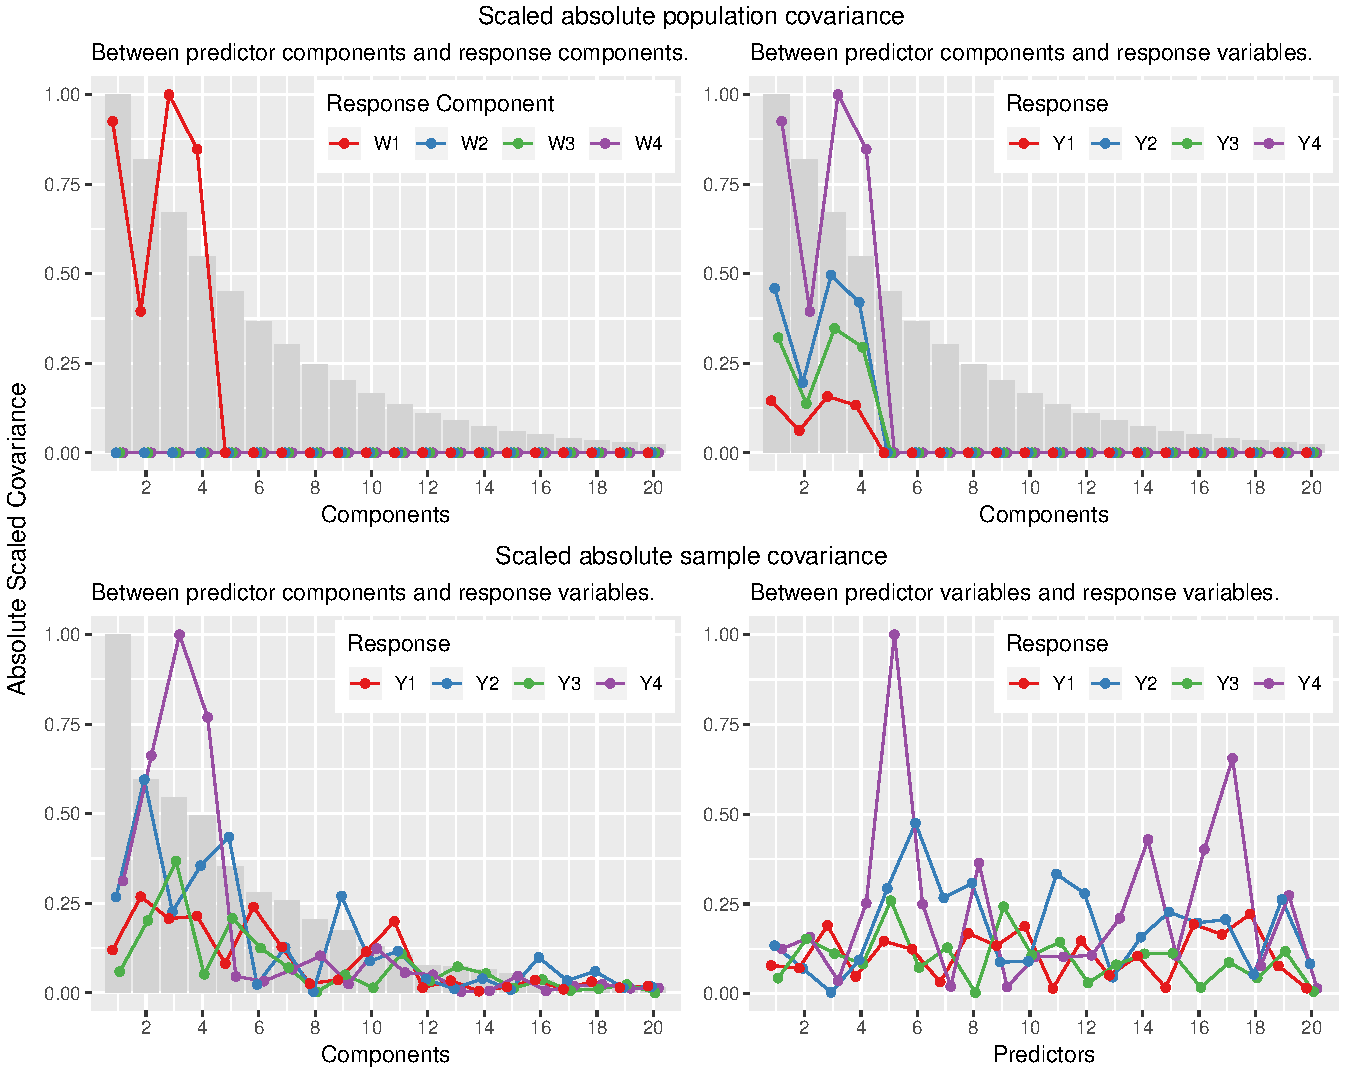
\includegraphics[width=1\linewidth]{main_files/figure-latex/est-cov-plot-1} \caption{Expected Scaled absolute covariance between predictor
components and response components (top left). Expected Scaled absolute
covariance between predictor components and response variables (top
right). Sample scaled absolute covariance between predictor components
and response variables (bottom left). Sample scaled absolute covariance
between predictor variables and response variables (bottom right). The
bar in the background are eigenvalues corresponding to each components
in population (top plots) and in sample (bottom plots).}\label{fig:est-cov-plot}
\end{figure}

The discussion here is made on the first design. A similar discussion
can be made on all 32 designs where each of the design holds the
properties of the data they simulate. These data are used by the
prediction methods discussed in previous section. Each prediction
methods are given independent dataset simulated in order to give them
equal opportunity to understand the dynamics in the data.

\hypertarget{basis-of-comparison}{%
\subsection{Basis of comparison}\label{basis-of-comparison}}

This study focuses mainly on the prediction performance of the methods
and emphasis specifically on the interaction between the properties of
the data, controlled by the simulation parameters, and the prediction
methods. The prediction performance is measured by the prediction error
for each response as in \eqref{eq:pred-error}. The prediction is the
theoretically computed expected prediction when the model is applied to
unseen observations corresponding to each response variable.

\begin{equation}
\text{prediction error}_j = \frac{1}{\sigma_{y_j|x}}\left[\left(\boldsymbol{\beta}_j - \boldsymbol{\hat{\beta}_j}\right)^t\boldsymbol{\Sigma}_{xx}\left(\boldsymbol{\beta}_j - \boldsymbol{\hat{\beta}_j}\right)\right] + 1
\label{eq:pred-error}
\end{equation} where, \(\boldsymbol{\Sigma}_{xx}\) is the true
covariance matrix of predictor and \(\sigma_{y_j\mid x}\) is the true
model error obtained from simulation of response \(j = 1, \ldots m\).
\highlight{Here prediction error is scaled by the true model error to remove its effect on prediction error.}
(\alert{Need better reason.}) The prediction error in
\eqref{eq:pred-error} is computed for all replications of 32 designs.

\hypertarget{exploration}{%
\section{Exploration}\label{exploration}}

The structure of final data for further analysis contains five factors
including the prediction methods and prediction error computed using
\eqref{eq:pred-error} corresponding to four responses using 0 to 10
predictor components for all 50 replications. Thus there are 32 (design)
\(\times\) 5 (methods) \(\times\) 11 (number of components) \(\times\)
50 (replications), i.e.~88000 observations. Here the variables
\texttt{Y1} to \texttt{Y4} corresponds to prediction error of response
variables.

Before performing any statistical analysis, this section tries to
explore some observed relationship between the prediction error, the
simulation parameters and the prediction methods. In the analysis onward
for each factor combination and replication, we will use two datasets:

\begin{itemize}
\tightlist
\item
  One with minimum prediction error that a method can give using
  arbitrary number of components (\emph{Error Dataset})
\item
  Another with the number of components that the method has used to give
  that minimum prediction error (\emph{Component Dataset})
\end{itemize}

Figure \ref{fig:pred-pca-hist-mthd-gamma-relpos} plots first two
principal components of \emph{error dataset} using columns from
\texttt{Y1} to \texttt{Y4}. Since higher prediction error results in
high scores the plot shows that the PCR, PLS1 and PLS2 methods are
influenced by two levels of position of relevant predictor components.
When the position of relevant predictors are at positon 5, 6, 7, 8, the
eigenvalues corresponding to them becomes smaller making those designs
difficult to model. However, the envelope methods have less influence of
\texttt{relpos} in this regard. In addition, the effect of
\texttt{gamma}, the level of multicollinearity, has less effect of all
cases. This indicates that the methods are somewhat reobust to handle
collinear predictors.

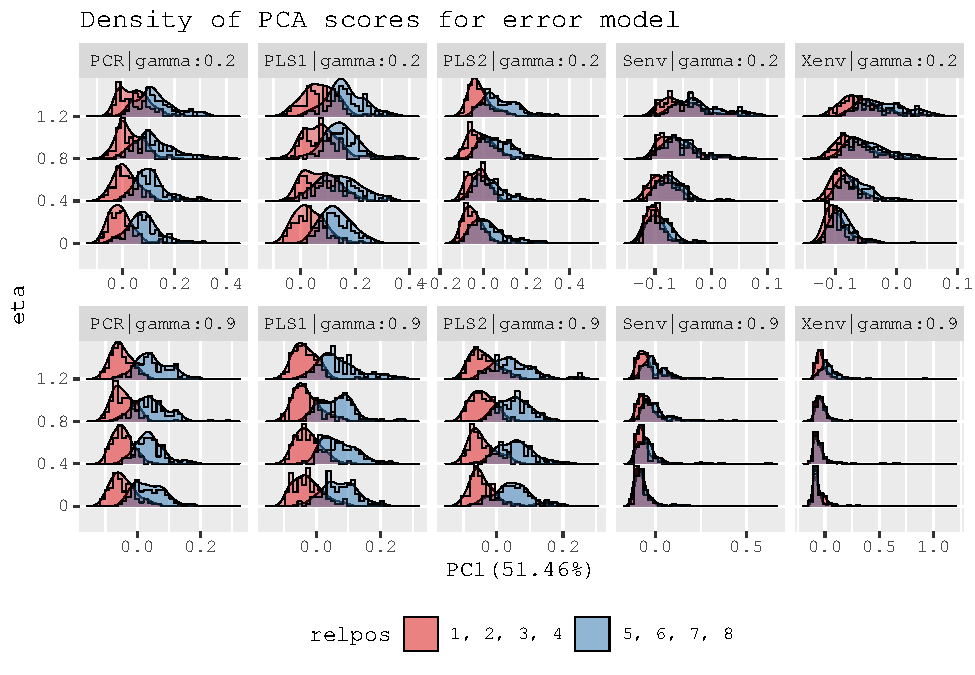
\includegraphics[width=1\linewidth]{main_files/figure-latex/pred-pca-hist-mthd-gamma-relpos-1}

\begin{itemize}
\tightlist
\item
  A similar interpretation as the previous plot can be made in the score
  density. In addition, higher correlation in response (controlled by
  \texttt{eta} parameter) yields in higher variation in the score of
  prediction error.
\item
  The plot in the right shows that the envelope methods are able to
  leverage the effect of correlation between the response while in case
  of others, the effect is similar in low and high correlation between
  the responses.
\end{itemize}

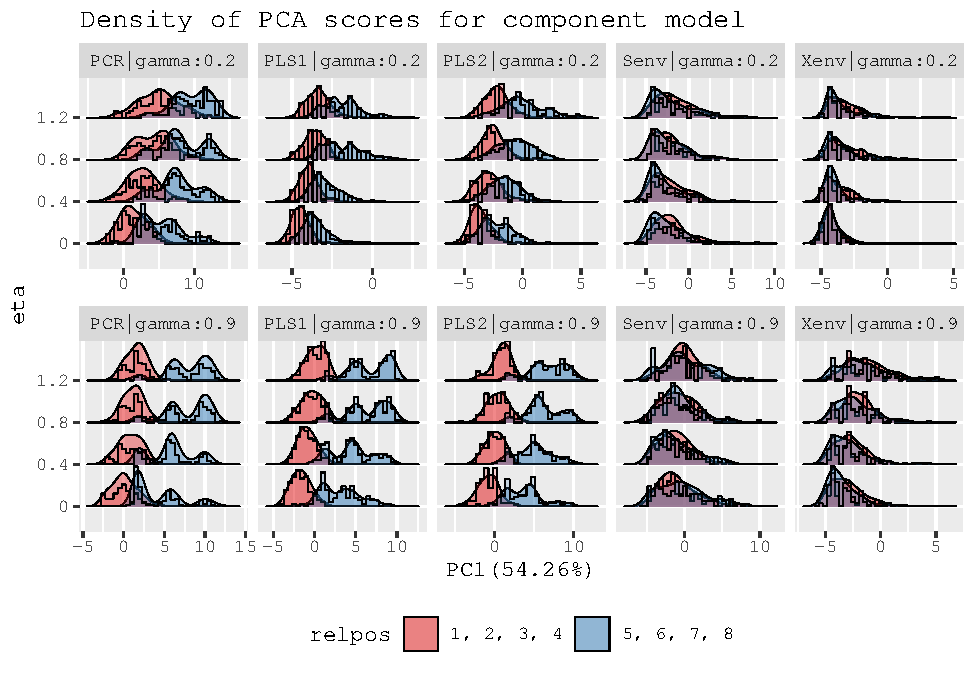
\includegraphics[width=1\linewidth]{main_files/figure-latex/comp-pca-hist-mthd-gamma-relpos-1}

\hypertarget{statistical-analysis}{%
\section{Statistical Analysis}\label{statistical-analysis}}

In order to carry out a proper statistical comparison, a multivariate
analysis of variance (MANOVA) is used with minimum prediction error
corresponding to each response variables for all design and their
replicates. The third order interaction of simulation parameters
(\texttt{p}, \texttt{gamma}, \texttt{eta} and \texttt{relpos}) and
\texttt{Methods} is used as independent factors as
\eqref{eq:expanded-model}.

\begin{equation}
\mathbf{y}_{abcdef} = \boldsymbol{\mu} + (\texttt{p}_a + \texttt{gamma}_b + \texttt{eta}_c + \texttt{relpos}_d + \texttt{Methods}_e)^3 + \boldsymbol{\varepsilon}_{abcdef}
\label{eq:expanded-model}
\end{equation}

where, \(\mathbf{y}_{abcdef}\) is a vector of prediction error for
factors,

\begin{itemize}
\tightlist
\item
  \(\texttt{p}_a =\) 20 and 250
\item
  \(\texttt{gamma}_b=\) 0.2 and 0.9
\item
  \(\texttt{eta}_c=\) 0, 0.4, 0.8 and 1.2
\item
  \(\texttt{relpos}_d=\) 1, 2, 3, 4 and 5, 6, 7, 8
\item
  \(\texttt{Methods}_e=\) \texttt{PCR}, \texttt{PLS1}, \texttt{PLS2},
  \texttt{Xenv} and \texttt{Senv}
\end{itemize}

In concise vector form, we can write as \eqref{eq:full-model}.

\begin{equation}
\mathbf{y} = \boldsymbol{\mu} + (\texttt{p} + \texttt{gamma} + \texttt{eta} + \texttt{relpos} + \texttt{Methods})^3 + \boldsymbol{\varepsilon}
\label{eq:full-model}
\end{equation} where, \(\mathbf{y}\) is the vector of prediction error
corresponding to response \(y_j, j = 1, \ldots 4\).

Prediction methods also varies on number of components they use to get
the minimum prediction error. A similar model as \eqref{eq:expanded-model}
is used with \(\mathbf{y}_{abcdef}\) as the number of components used to
get the minimum prediction error. Here Pellai's trace is used for
evaluating these model.

\begin{figure}
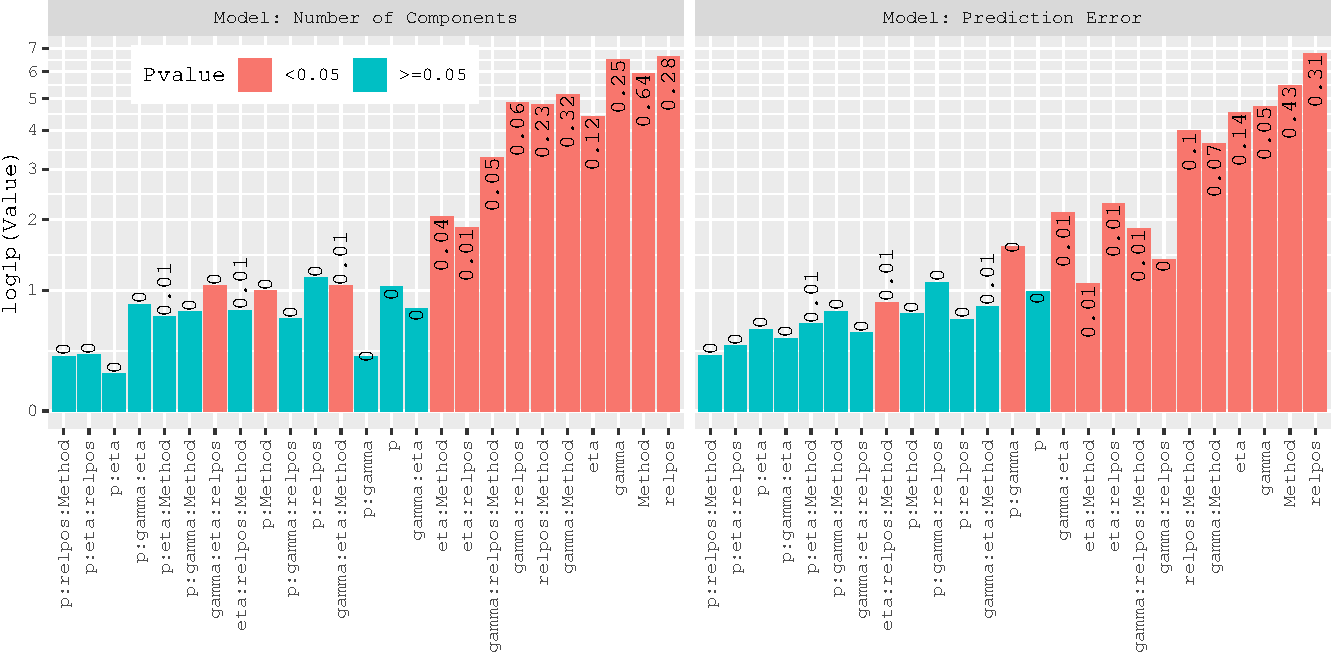
\includegraphics[width=1\linewidth]{main_files/figure-latex/prediction-model-plot-1} \caption{Pillai Statistic and F-value for the MANOVA model. The bar represents the F-value and the text labels are Pillai Statistic for corresponding factor.}\label{fig:prediction-model-plot}
\end{figure}

SOME OBSERVATIONS:

\begin{itemize}
\tightlist
\item
  All main effects except \texttt{p} are significant and has large
  effect on both minimum number of components and prediction error.
\item
  Position of relevant components have largest effect on prediction
  error. In case of minimum number of components, multicollineary also
  have largest effect in addition to the position of relevant
  components.
\item
  However based on pillai trace statistic, Method has the lastest effect
  on both of the model.
\item
  The interactions \texttt{p:gamma} and \texttt{eta:relpos:Method} is
  significant in prediction error model but not in minim number of
  components model. However, all of these interactions have small pillai
  statistic.
\item
  In case of Number of components model interaction effects
  \texttt{gamma:eta:Method}, \texttt{p:Method} and
  \texttt{gamma:eta:relpos} are significant but not in the case of
  prediciton error model. Similar to previous point, they too have small
  pillai statistic.
\end{itemize}

\hypertarget{effect-analysis}{%
\subsection{Effect Analysis}\label{effect-analysis}}

ON PREDICTION ERROR MODEL:

\begin{itemize}
\tightlist
\item
  It would be desirable to observe effect of these interactions. Figure
  \ref{fig:pred-eff-plots} (left) shows clear difference of \texttt{eta}
  for a given \texttt{relpos}. The plot also shows a clear difference in
  effect of methods on prediction error.
\item
  Figure \ref{fig:pred-eff-plots} (right) shows effect of \texttt{gamma}
  for a given \texttt{method} and \texttt{eta}. It shows that these
  methods gives low prediction error is high multicollinear situations.
\end{itemize}

\begin{figure}
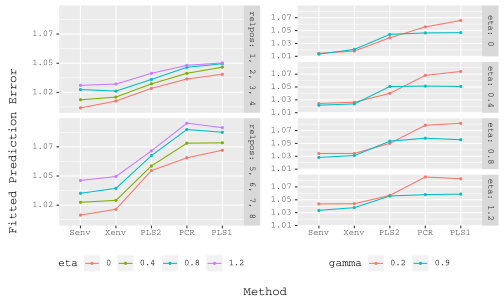
\includegraphics[width=1\linewidth]{main_files/figure-latex/pred-eff-plots-1} \caption{Effect plot of some interactions of the multivariate linear model}\label{fig:pred-eff-plots}
\end{figure}

ON MINIMUM NUMBER OF COMPONENTS MODEL:

\begin{itemize}
\tightlist
\item
  Figure \ref{fig:comp-eff-plots} (left) shows that \texttt{xenv} has
  used minimum number of components followed by \texttt{senv} methods
  than others in order to get their minimum prediction error.
\item
  The same figure also suggest that the minimum number of components
  used by \texttt{PLS1}, \texttt{PLS2} and \texttt{PCR} vary and has
  high effect of \texttt{eta}. The \texttt{senv} model which consider
  both X and Y correlation structure while estimating regression
  coefficients has smallest variation of number of components used for
  different \texttt{eta} parameters.
\item
  Figure \ref{fig:comp-eff-plots} (right) shows that in case of low
  multicollinearity in the model \texttt{PLS} methods are used less
  number of components than \texttt{PCR}. This is expected since,
  \texttt{PLS} methods consider the covariance structure of predictor
  and response which \texttt{PCR} does not.
\end{itemize}

\begin{figure}
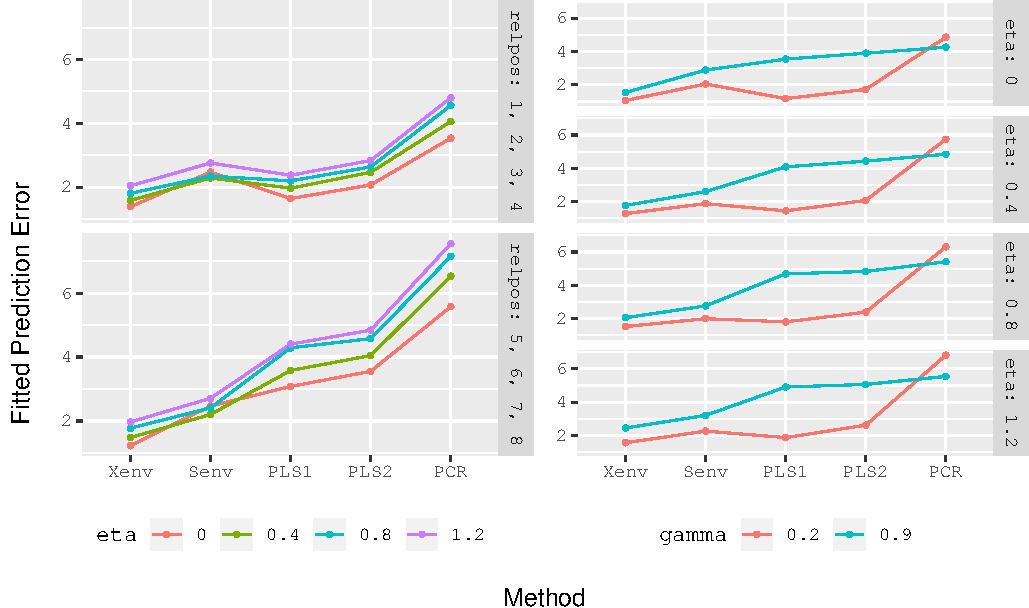
\includegraphics[width=1\linewidth]{main_files/figure-latex/comp-eff-plots-1} \caption{Effect plot of some interactions of the multivariate linear model}\label{fig:comp-eff-plots}
\end{figure}

ADDITIONAL OBSERVATIONS:

\begin{itemize}
\tightlist
\item
  Place for variable selection
\item
  A PLS model is used to cross-validate the effects of these factors.
  The loading plot for the same model but only with second order
  interaction is in figure \ref{fig:pls-loadings}.
\end{itemize}

\hypertarget{a-partial-least-square-analysis-on-the-model}{%
\subsection{A partial least square analysis on the
model}\label{a-partial-least-square-analysis-on-the-model}}

\begin{figure}
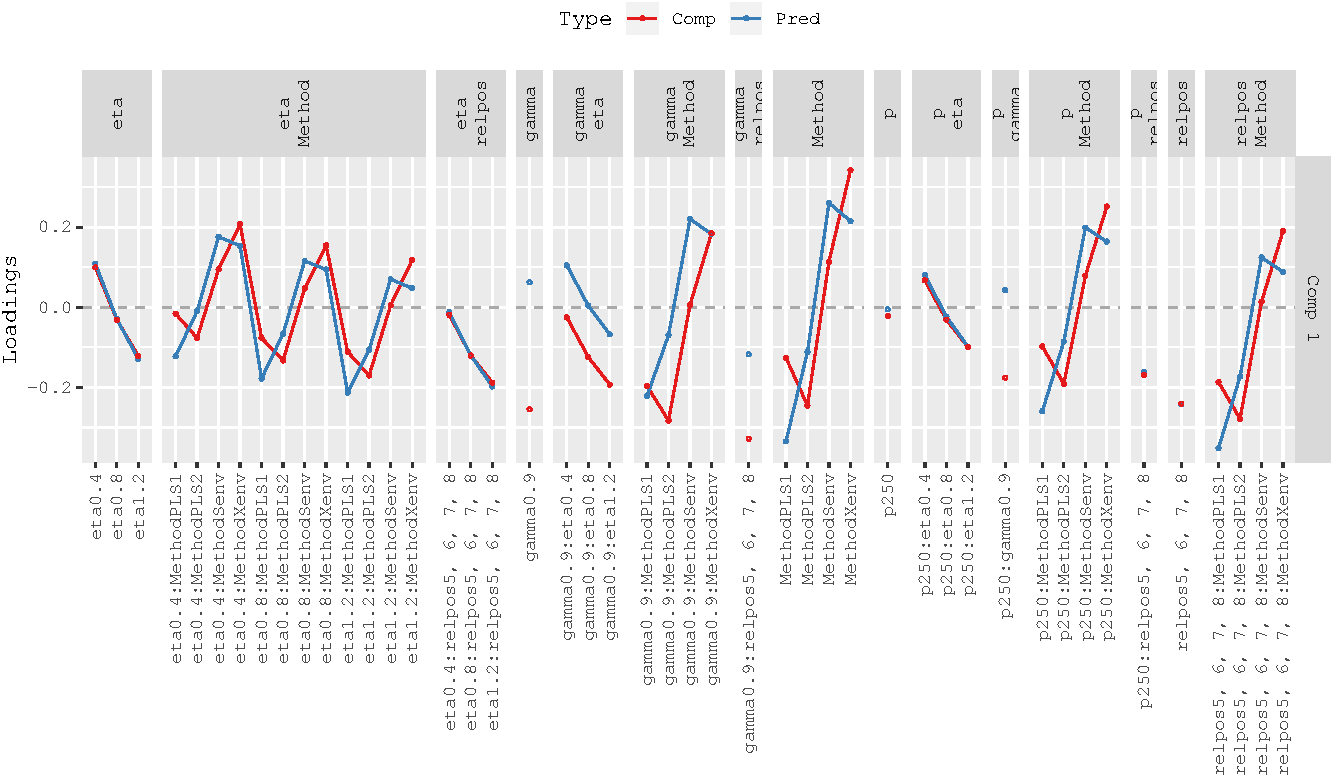
\includegraphics[width=1\linewidth]{main_files/figure-latex/pls-loadings-1} \caption{PLS Loadings (Component 1)}\label{fig:pls-loadings}
\end{figure}

SOME OBSERVATIONS:

\begin{itemize}
\tightlist
\item
  The loadings for first components plotted in
  Figure-\ref{fig:pls-loadings} has clearly separated the envelope
  models from the rest by giving positive loading for them and negative
  for the rest.
\item
  This components has only explained 7.969 in prediction error model and
  7.697 in minimum components model.
\end{itemize}

CONFUSION:

\begin{itemize}
\tightlist
\item
  The explained variation by each of these components is not in
  decending order as each successive components of PLS model is supposed
  to explain the maximum covarinace between predictor and response.
\end{itemize}

\hypertarget{refs}{}

\hypertarget{appendix-appendix-a}{%
\appendix}



\renewcommand\refname{References}
\bibliography{ref-db.bib}


\end{document}
